\chapter{Resultados}

A continuación vamos a plantear algunos casos de estudio para analizar en detalle el comportamiento del algoritmo.
Para este análisis utilizaremos la estrategia Síntesis - Nueva acción.

\section{Laberinto de 25 posiciones}

El primer entorno que presentamos es un laberinto de 25 posiciones. En cada posición el robot puede tener hasta 4
acciones disponibles, las cuales son norte, sur, este y oeste. El entorno no tiene agentes externos. El objetivo de
este caso de estudio es ver como el robot encuentra la salida en un laberinto complejo sin información previa.

\begin{figure}[H]
	\centering
		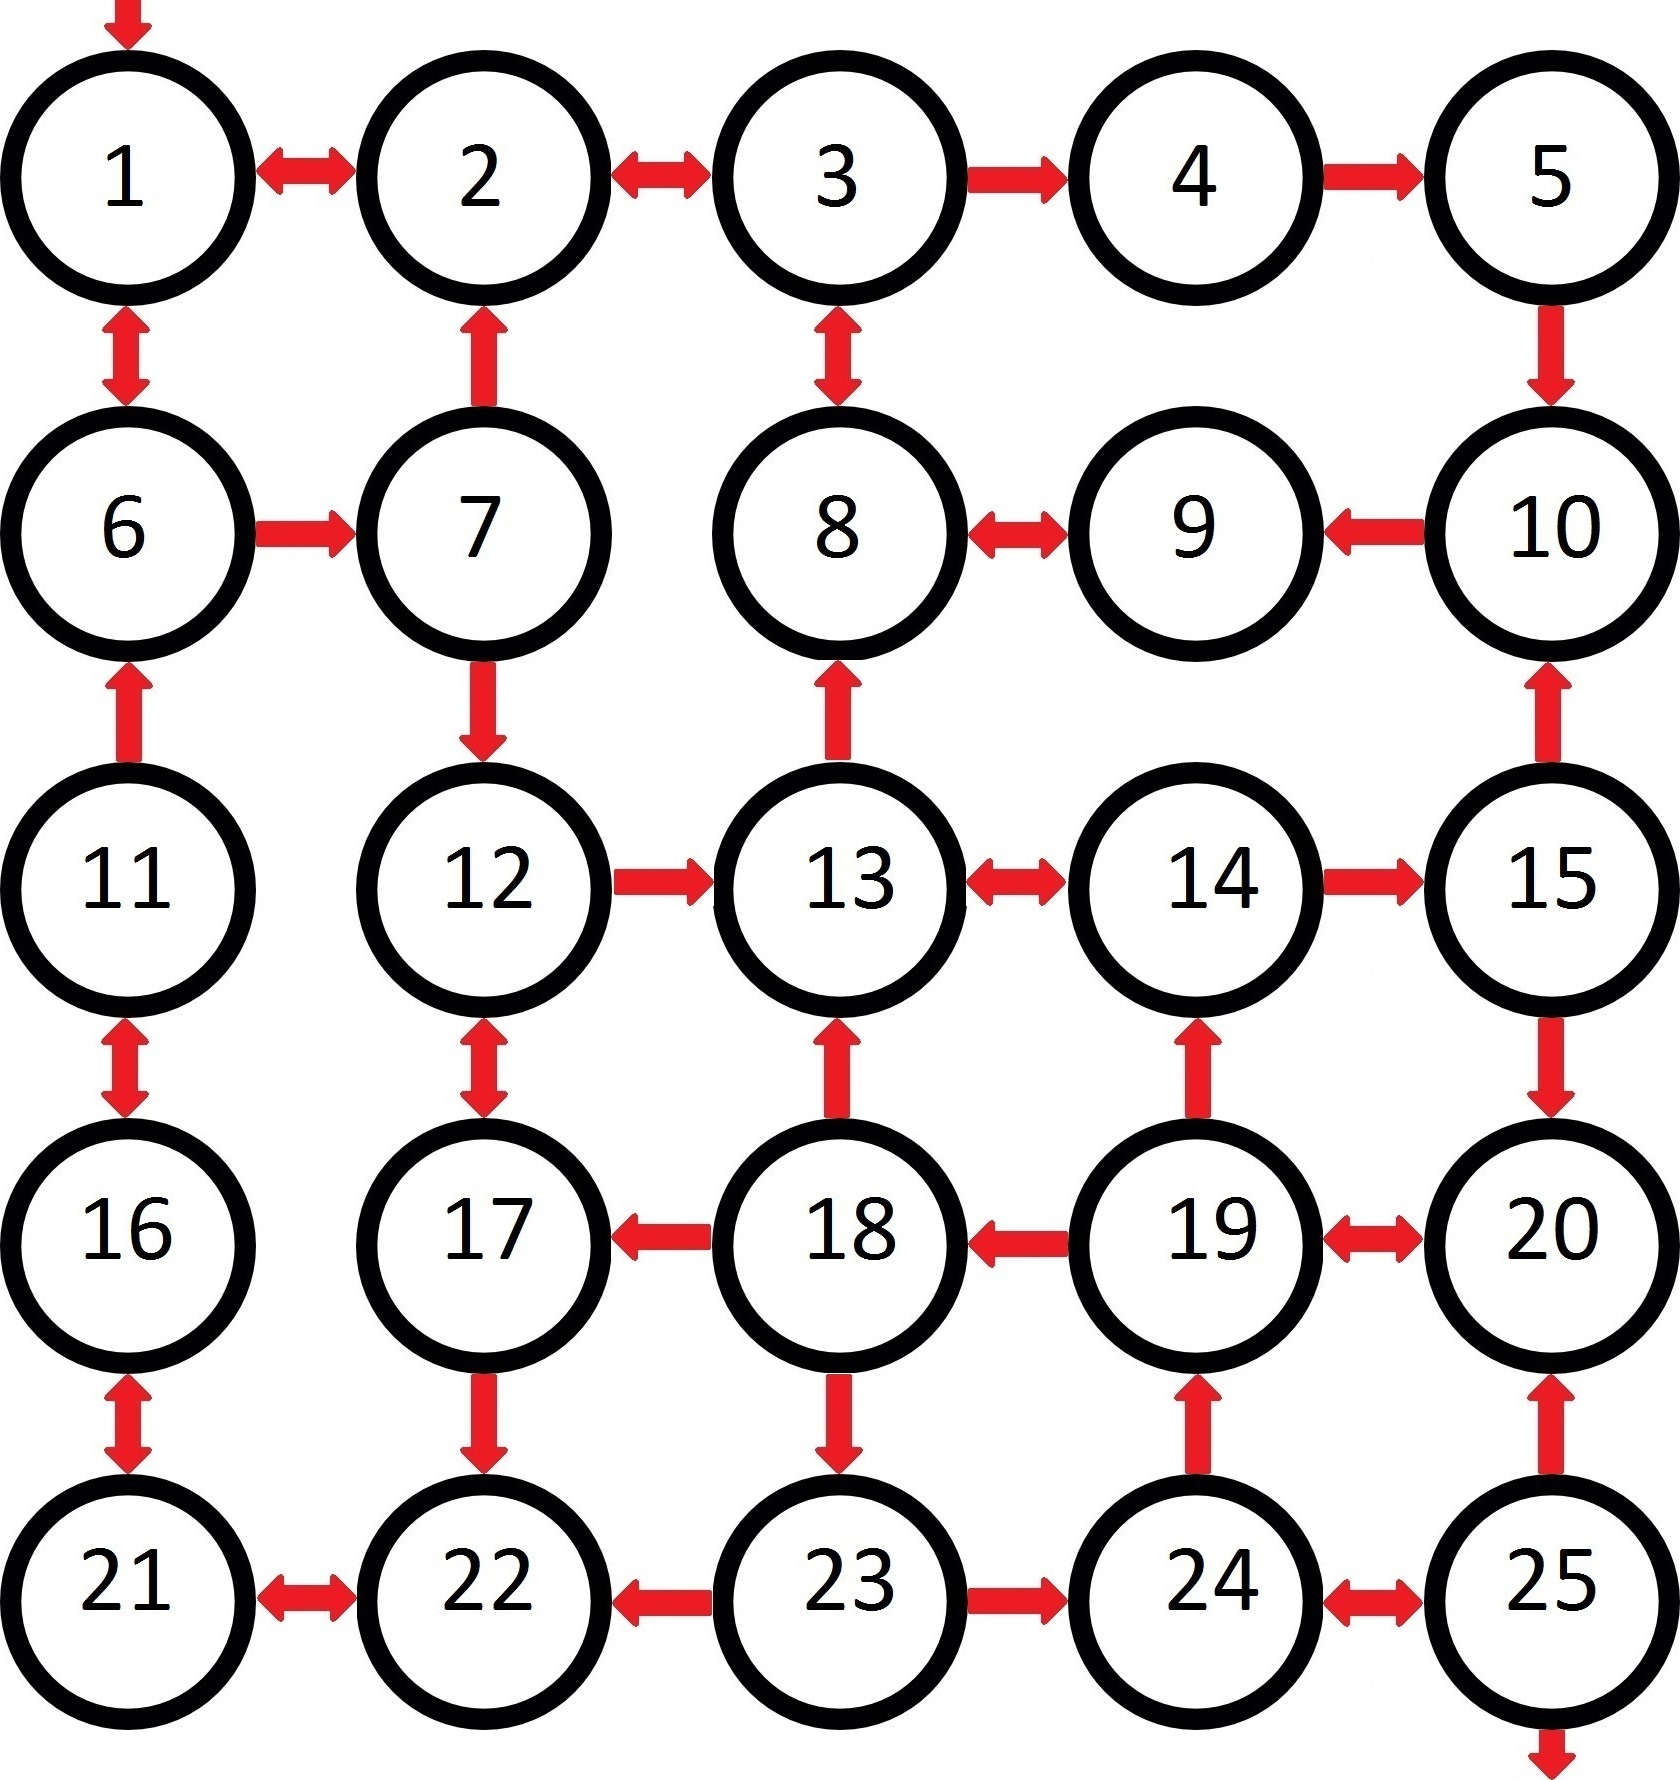
\includegraphics[width=0.9\textwidth]{Imagenes/Laberintos/25.jpg}
	\caption{Laberinto de 25 posiciones}
	\label{fig:25}
\end{figure}

\subsection{Especificación en MTSA}

\begin{Code}[commandchars=&\[\]]
&fvtextcolor[0000A0][VIEW] = &fvtextcolor[0000A0][P01],
&fvtextcolor[0000A0][P01]  = (sur   -> &fvtextcolor[0000A0][P06] | este  -> &fvtextcolor[0000A0][P02]),
&fvtextcolor[0000A0][P02]  = (este  -> &fvtextcolor[0000A0][P03] | oeste -> &fvtextcolor[0000A0][P01]),
&fvtextcolor[0000A0][P03]  = (sur   -> &fvtextcolor[0000A0][P08] | este  -> &fvtextcolor[0000A0][P04] | oeste -> &fvtextcolor[0000A0][P02]),
&fvtextcolor[0000A0][P04]  = (este  -> &fvtextcolor[0000A0][P05]),
&fvtextcolor[0000A0][P05]  = (sur   -> &fvtextcolor[0000A0][P10]),
&fvtextcolor[0000A0][P06]  = (norte -> &fvtextcolor[0000A0][P01] | este  -> &fvtextcolor[0000A0][P07]),
&fvtextcolor[0000A0][P07]  = (norte -> &fvtextcolor[0000A0][P02] | sur   -> &fvtextcolor[0000A0][P12]),
&fvtextcolor[0000A0][P08]  = (norte -> &fvtextcolor[0000A0][P03] | este  -> &fvtextcolor[0000A0][P09]),
&fvtextcolor[0000A0][P09]  = (oeste -> &fvtextcolor[0000A0][P08]),
&fvtextcolor[0000A0][P10]  = (oeste -> &fvtextcolor[0000A0][P09]),
&fvtextcolor[0000A0][P11]  = (norte -> &fvtextcolor[0000A0][P06] | sur   -> &fvtextcolor[0000A0][P16]),
&fvtextcolor[0000A0][P12]  = (sur   -> &fvtextcolor[0000A0][P17] | este  -> &fvtextcolor[0000A0][P13]),
&fvtextcolor[0000A0][P13]  = (norte -> &fvtextcolor[0000A0][P08] | este  -> &fvtextcolor[0000A0][P14]),
&fvtextcolor[0000A0][P14]  = (este  -> &fvtextcolor[0000A0][P15] | oeste -> &fvtextcolor[0000A0][P13]),
&fvtextcolor[0000A0][P15]  = (norte -> &fvtextcolor[0000A0][P10] | sur   -> &fvtextcolor[0000A0][P20]),
&fvtextcolor[0000A0][P16]  = (norte -> &fvtextcolor[0000A0][P11] | sur   -> &fvtextcolor[0000A0][P21]),
&fvtextcolor[0000A0][P17]  = (norte -> &fvtextcolor[0000A0][P12] | sur   -> &fvtextcolor[0000A0][P22]),
&fvtextcolor[0000A0][P18]  = (norte -> &fvtextcolor[0000A0][P13] | sur   -> &fvtextcolor[0000A0][P23] | oeste -> &fvtextcolor[0000A0][P17]),
&fvtextcolor[0000A0][P19]  = (norte -> &fvtextcolor[0000A0][P14] | este  -> &fvtextcolor[0000A0][P20] | oeste -> &fvtextcolor[0000A0][P18]),
&fvtextcolor[0000A0][P20]  = (oeste -> &fvtextcolor[0000A0][&fvtextcolor[0000A0][P19]]),
&fvtextcolor[0000A0][P21]  = (norte -> &fvtextcolor[0000A0][P16] | este  -> &fvtextcolor[0000A0][P22]),
&fvtextcolor[0000A0][P22]  = (oeste -> &fvtextcolor[0000A0][P21]),
&fvtextcolor[0000A0][P23]  = (este  -> &fvtextcolor[0000A0][P24] | oeste -> &fvtextcolor[0000A0][P22]),
&fvtextcolor[0000A0][P24]  = (norte -> &fvtextcolor[0000A0][&fvtextcolor[0000A0][P19]] | este  -> &fvtextcolor[0000A0][P25]),
&fvtextcolor[0000A0][P25]  = (norte -> &fvtextcolor[0000A0][P20] | oeste -> &fvtextcolor[0000A0][P24] | salir -> &fvtextcolor[0000A0][P25]).

&fvtextcolor[0000A0][MODEL] = (norte? -> &fvtextcolor[0000A0][MODEL] | sur?   -> &fvtextcolor[0000A0][MODEL] | este? -> &fvtextcolor[0000A0][MODEL] | 
         oeste? -> &fvtextcolor[0000A0][MODEL] | salir? -> &fvtextcolor[0000A0][MODEL]).

&fvtextcolor[0000FF][set] &fvtextcolor[0000A0][Controllable_25] = {norte, sur, este, oeste, salir}
&fvtextcolor[0000FF][fluent] &fvtextcolor[0000A0][F_Salir]      = <salir, &fvtextcolor[0000A0][Controllable_25]\{salir}>
&fvtextcolor[0000FF][assert] &fvtextcolor[0000A0][A_Salir]      = &fvtextcolor[0000A0][F_Salir]

&fvtextcolor[0000FF][controllerSpec] &fvtextcolor[0000A0][GOAL_25] = {
    liveness     = {&fvtextcolor[0000A0][A_Salir]}
    controllable = {&fvtextcolor[0000A0][Controllable_25]}
}

&fvtextcolor[0000FF][exploration] &fvtextcolor[0000A0][M25] = {
    environment = {&fvtextcolor[0000A0][VIEW]},
    model       = {&fvtextcolor[0000A0][MODEL]},
    goal        = {&fvtextcolor[0000A0][GOAL_25]}
}
\end{Code}

\subsection{Análisis preliminar}

El robot logra salir del laberinto en 116 pasos, pasando en promedio 4.64 veces por cada posición.
Podemos observar a simple vista que las posiciones más visitadas forman parte del camino hacia la salida.

\begin{figure}[H]
	\centering
		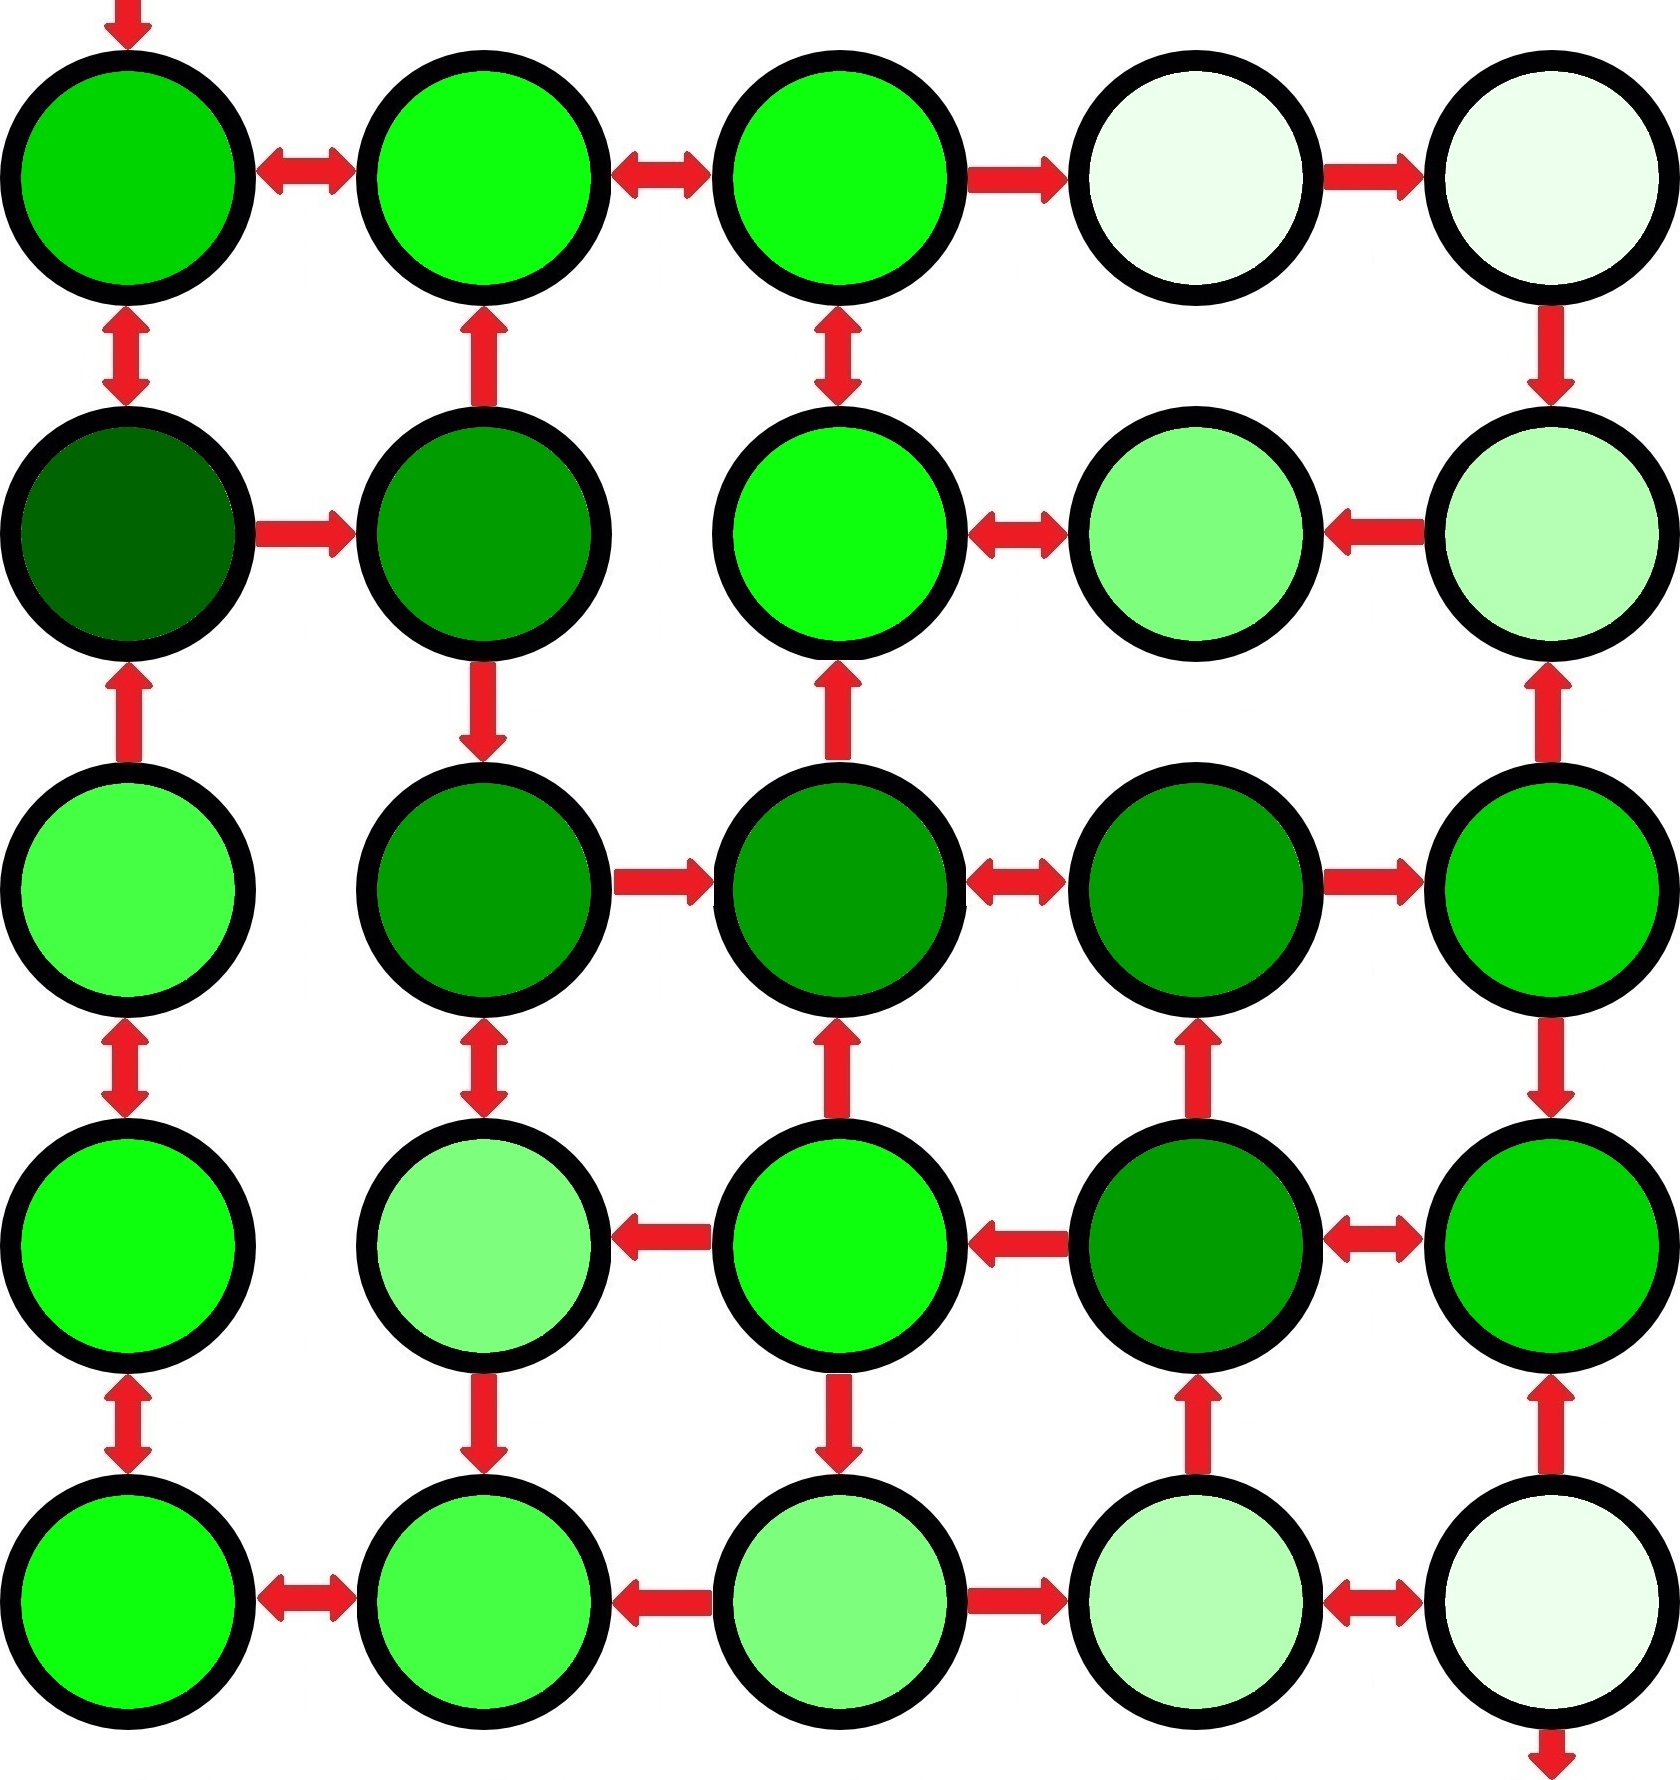
\includegraphics[width=1.0\textwidth]{Imagenes/Laberintos/25_calor.jpg}
	\caption{Mapa de calor del robot en el laberinto de 25 posiciones}
	\label{fig:25_calor}
\end{figure}

\clearpage

\subsection{Análisis de los modelos}

Para lograr dar una respuesta sobre si es posible o no garantizar el cumplimiento del objetivo fue necesario
explorar el entorno casi por completo. Las únicas dos acciones no ejecutadas fueron norte y oeste desde la posición
final, por lo cual en el modelo del conocimiento van hacia \textit{La nube}.

\begin{figure}[H]
	\centering
		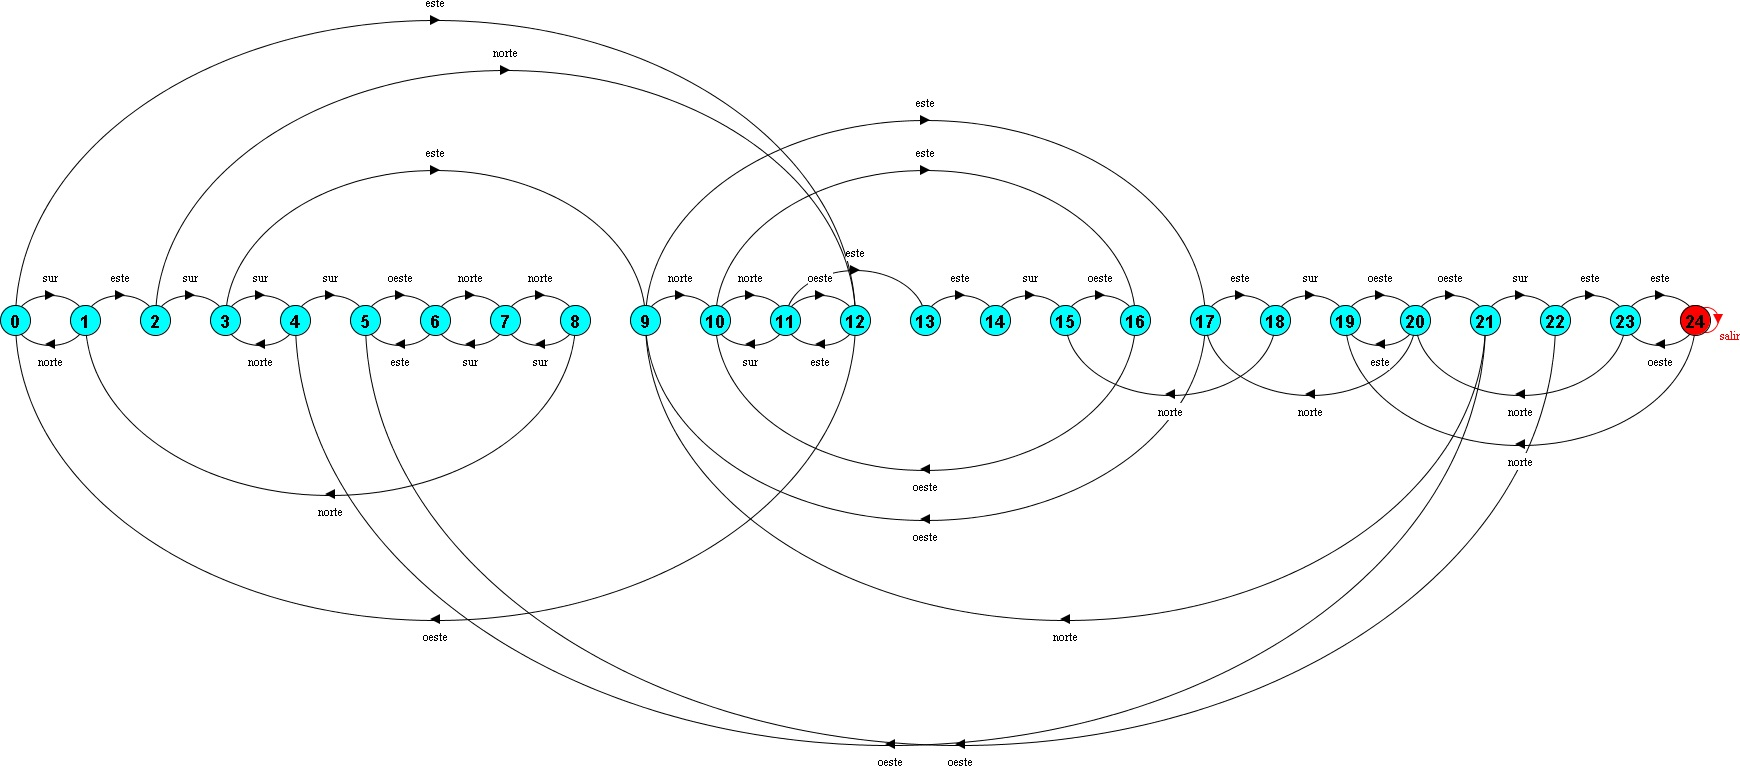
\includegraphics[width=1.0\textwidth]{Imagenes/Laberintos/25_view.jpg}
	\caption{LTS que representa al mapa del laberinto de 25 posiciones}
	\label{fig:25_view}
\end{figure}

\begin{figure}[H]
	\centering
		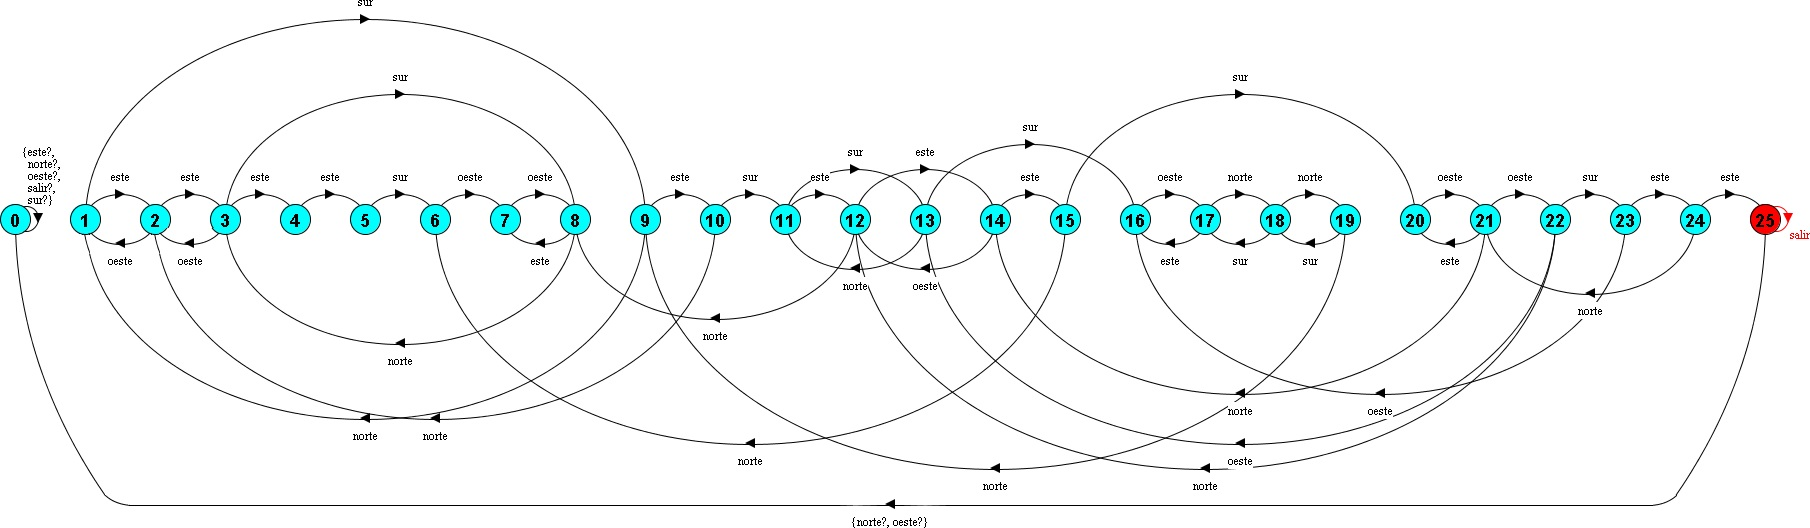
\includegraphics[width=1.0\textwidth]{Imagenes/Laberintos/25_knowledge.jpg}
	\caption{MTS que representa al conocimiento adquirido sobre el laberinto de 25 posiciones}
	\label{fig:25_knowledge}
\end{figure}

\clearpage

\subsection{Variantes}

Si eliminamos la acción salir, el robot descubre que el laberinto no tiene salida en 122 pasos, formando un modelo
de conocimiento en cual una de sus dos componentes conexas es bisimilar al LTS que representa al mapa, siendo su
otra componente conexa \textit{La nube}.

\vspace{\baselineskip}
Si modificamos el mapa para que la acción salir se encuentre en \textcolor[HTML]{0000A0}{P08} en vez de en \textcolor[HTML]{0000A0}{P25},
el robot logra salir del laberinto en tan solo 9 pasos, siendo su modelo del conocimiento mucho más reducido que el modelo del mapa.

\begin{figure}[H]
	\centering
		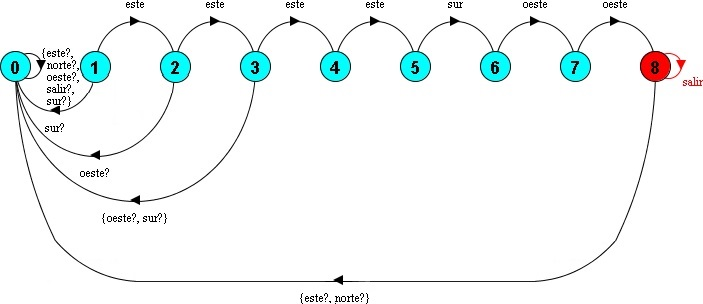
\includegraphics[width=1.0\textwidth]{Imagenes/Laberintos/25_knowledge_alternativo.jpg}
	\caption{MTS que representa al conocimiento adquirido sobre el laberinto de 25 posiciones con salida en la posición 8}
	\label{fig:25_knowledge_alternativo}
\end{figure}